
\documentclass{article}
\usepackage[top=1in, bottom=1in, left=1.25in, right=1.25in]{geometry}
\renewcommand{\baselinestretch}{2} 
\usepackage{amsmath,amssymb}
\usepackage{xcolor}
\usepackage{graphicx}
\setlength{\parindent}{0pt}
\usepackage[utf8]{inputenc}
\usepackage{parskip}
\usepackage{indentfirst}
 
\usepackage{listings}
\usepackage{color}
\usepackage{longtable}
 
\definecolor{codegreen}{rgb}{0,0.6,0}
\definecolor{codegray}{rgb}{0.5,0.5,0.5}
\definecolor{codepurple}{rgb}{0.58,0,0.82}
\definecolor{backcolour}{rgb}{0.95,0.95,0.92}
 
\lstdefinestyle{mystyle}{
    backgroundcolor=\color{backcolour},   
    commentstyle=\color{codegreen},
    keywordstyle=\color{magenta},
    numberstyle=\tiny\color{codegray},
    stringstyle=\color{codepurple},
    basicstyle=\footnotesize,
    breakatwhitespace=false,         
    breaklines=true,                 
    captionpos=b,                    
    keepspaces=true,                 
    numbers=left,                    
    numbersep=5pt,                  
    showspaces=false,                
    showstringspaces=false,
    showtabs=false,                  
    tabsize=2
}
 
\lstset{style=mystyle}
\usepackage{hyperref}

\title{Bios/CS 534 Project 2}
\author{Chenxi Cai}
\begin{document}
\lstset{numbers=left, numberstyle=\small, keywordstyle=\color{blue!70}, commentstyle=\color{red!50!green!50!blue!50}, frame=shadowbox, rulesepcolor=\color{red!20!green!20!blue!20},escapeinside=``, xleftmargin=2em,xrightmargin=2em, aboveskip=1em}
\maketitle

\section{Abstract}
In this final project, a dataset of 1000 samples with 120 proteins features came from the blood plasma of some patients and controls. Some techniques were used to analyze this dataset in order to develop blood protein biomarkers for a certain type of cancer. First, the Principal component analysis (PCA) was used for dimension reduction and the visualizations showed there appeared to be subgroups of proteins, whereas no subgroups of samples. Then Bayesian Information Criterion (BIC) estimated the number of clusters in K-Means and AgglomerativeClustering clustering techniques. These two methods have similar results after clustering the proteins. Finally, the dataset was split in a 3:1:1 ratio into training, validation, and testing sets. Four classifiers:  KNeighborsClassifier, RandomForestClassifier, GradientBoostingClassifier and LogisticRegressionCV were tuned with cross-validation GridSearchCV using the training data and GradientBoostingClassifier is the best one based on its performance on the validation data. Then I evaluated the model with GradientBoostingClassifier and got the error rate 0.3. I also got the conclusion, based on feature importance ranking, that protein 74th, 34th and 54th are the top predictors. 

\section{Methods}
\subsection{Dimension Reduction Technique }
I used Principal component analysis (PCA) technique here. It is a linear dimensionality reduction using Singular Value Decomposition of the data to project it to a lower dimensional space.\cite{halko2011finding} The class is $''sklearn.decomposition.PCA''$ and the parameter neededs to set is the 
\textbf{n\_components}, which is number of components to keep. Here we set n\_components $= 2$.


\subsection{Clustering}
K-means and AgglomerativeClustering were applied here. The KMeans algorithm clusters data by trying to separate samples in n groups of equal variance, minimizing a criterion known as the inertia or within-cluster sum-of-squares.\cite{arthur2007k}. Hierarchical clustering is a general family of clustering algorithms that build nested clusters by merging or splitting them successively.\cite{rokach2005clustering} The AgglomerativeClustering object performs a hierarchical clustering using a bottom up approach: each observation starts in its own cluster, and clusters are successively merged together. These two algorithms require the number of clusters to be specified. The classes are $"sklearn.cluster.KMeans"$ and  $"sklearn.cluster.AgglomerativeClustering"$. The parameter of the number of clusters is \textbf{n\_clusters}. I used Bayesian Information Criterion (BIC) method to visualize the data character and then determined the number of clusters K. As shown in Fig.~\ref{bic}, the number of clusters should be set to 3. n\_clusters $= 3$.

\begin{figure}[h]
    		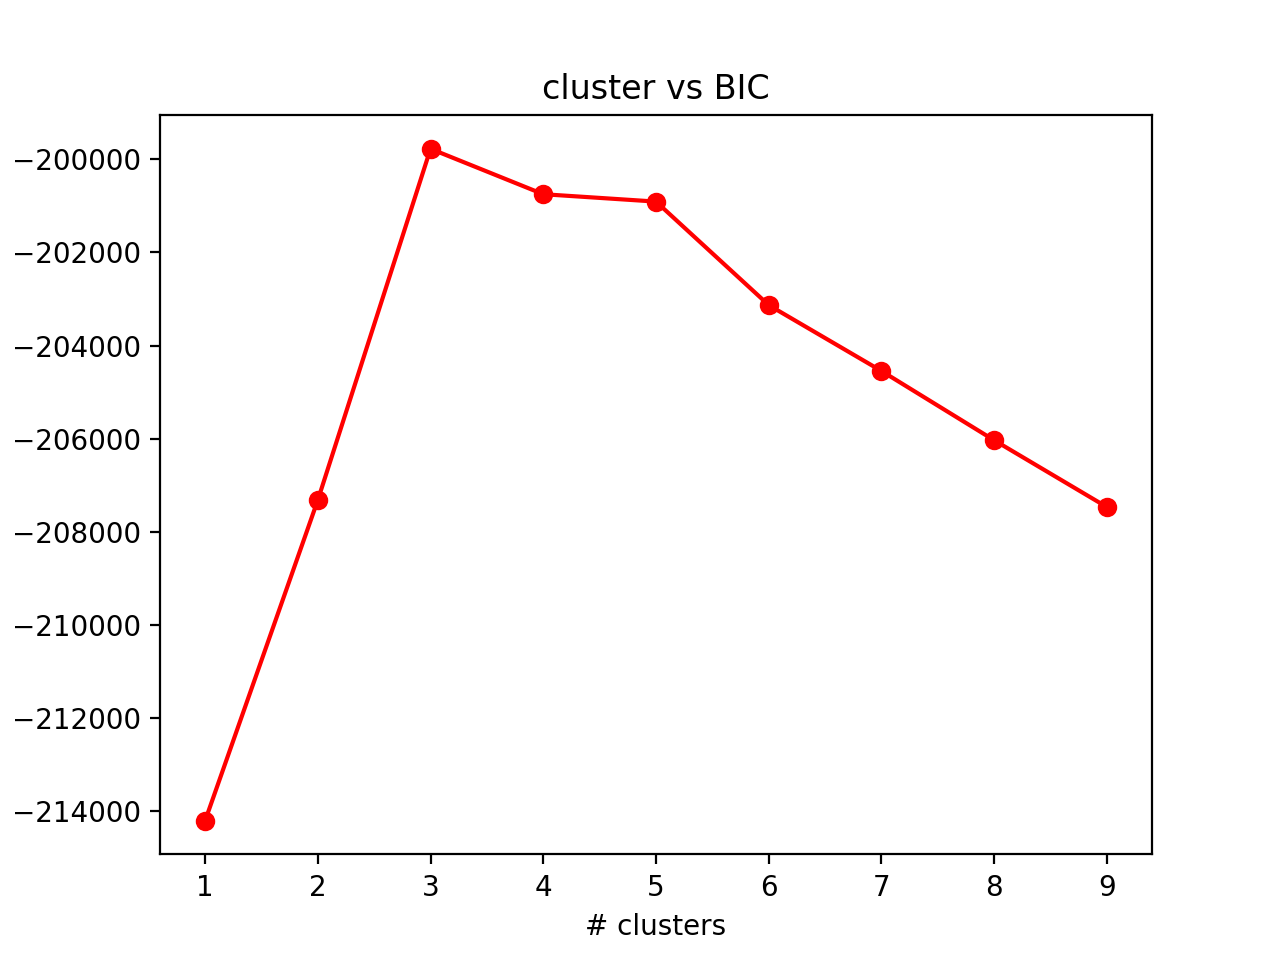
\includegraphics[width=5 in]{BIC.png}
		\centering
		\caption{Plots of BIC}
		\label{bic}
    		\end{figure}


\subsection{Classifier}
The dataset was split in a 3:1:1 ratio into training, validation, and testing sets. With training data and GridSearchCV cross-validation method, I tuned KNeighborsClassifier, RandomForestClassifier and GradientBoostingClassifier. The GridSearchCV is an exhaustive search over specified parameter values for an estimator.\cite{bergstra2012random} Neighbors-based classification is a type of instance-based learning or non-generalizing learning: it does not attempt to construct a general internal model, but simply stores instances of the training data.\cite{bentley1975multidimensional} RandomForestClassifier is a meta estimator that fits a number of decision tree classifiers on various sub-samples of the dataset and use averaging to improve the predictive accuracy and control over-fitting.\cite{breiman2001random} GradientBoostingClassifier builds an additive model in a forward stage-wise fashion; it allows for the optimization of arbitrary differentiable loss functions.\cite{friedman2001greedy}  The best parameters after tuning of each classifiers are list in Table.\ref{best_para}. The parameter \textbf{cv} is set to 10 for all classifiers. 

 \begin{table}[h!]
 \centering
 \caption{Best Parameters of Each Classifiers}
 \label{best_para}
\begin{tabular}{  | c | c |   }


\hline
Classifier & best parameter  \\
\hline
KNeighborsClassifier & n\_neighbors=2 \\
\hline
RandomForestClassifier & n\_estimators=510 \\
\hline
GradientBoostingClassifier & learning\_rate=0.52 \\
\hline
 \end{tabular}
\end{table}

The tuning procedure and selection of parameters is in Supplementary File 1. 

I also use LogisticRegressionCV classifier\cite{schmidt2017minimizing}, the class is $"sklearn.linear\_model.LogisticRegressionCV"$ and the parameter \textbf{cs} is set by default to be ten values in a logarithmic scale between 1e-4 and 1e4. 


\section{Results and Discussion}
\subsection{Dimension Reduction Technique }
With PCA, I did twice (a) for the samples; (b) for the proteins. And the 2-dimensional visualizations of them are shown in Fig.~\ref{sample_v} and Fig.~\ref{protein_v}, separately. From Fig.~\ref{sample_v}, we can know that there appears to be no subgroups of sample. All the points are messy. However, from Fig.~\ref{protein_v} we can see that there are three main subgroups of proteins and the points in center may be noise points. Those subgroups are not associated with the clinical outcome because the outcomes are binary values and there are only two classes, while there appears three subgroups in proteins.

\begin{figure}[h]
    		\includegraphics[width=5 in]{dimension_reduction.png}
		\centering
		\caption{Dimension Reduction Visualization of Samples }
		\label{sample_v}
    		\end{figure}
		
\begin{figure}[h]
    		\includegraphics[width=5 in]{dimension_reduction_reve.png}
		\centering
		\caption{Dimension Reduction Visualization of Proteins }
		\label{protein_v}
    		\end{figure}

\subsection{Clustering}
By calculating BIC values, we set the number of cluster K 	to 3 in K-means and AgglomerativeClustering, which is shown in Fig.~\ref{bic}. The predict labels of proteins are shown in Table.\ref{lables_cluster}.

\begin{table}[h!]
\centering

\caption{120 Predicted Labels of Kmeans and AgglomerativeClustering}
\label{lables_cluster} 
\begin{tabular}{  | c | c | c |  }	
\hline
numbers & Kmeans  & Agglomerative \\
\hline
1 & 1 & 2 \\
\vdots & \vdots & \vdots \\
38 & 1  & 2 \\
39 & 2  & 1 \\
\vdots & \vdots  & \vdots \\
76 & 2  & 1 \\
78 & 0 & 0 \\
\vdots & \vdots  & \vdots \\
\color{red}117 & \color{red}1 &\color{red} 0\\
118 & 0  & 0 \\
\vdots & \vdots  & \vdots \\
120 & 0  & 0\\

\hline

\end{tabular}
\end{table}

Only 117th protein is clustered in different clusters by Kmeans and AgglomerativeClustering. The two methods yield very similar results.

\subsection{Classifier}
After tuning each KNeighborsClassifier, RandomForestClassifier and GradientBoostingClassifier with cross-validation using the training data, the feature rankings of RandomForestClassifier and GradientBoostingClassifier are show in Table.~\ref{rank}. We can know that the 74th, 34th and 54th proteins are the top predictors.

I also used  LogisticRegressionCV classifier. The scores of validation data based on all these four classifiers are listed in Table.~\ref{vali}. We can draw the conclusion that GradientBoostingClassifier is the best classifier.

Then using the testing data, the performance of the GradientBoostingClassifier can be showed by score, which is 0.7. So the error rate is 0.3.

\begin{table}[h!]
\centering

\caption{Scores of Four Classifiers}
\label{vali} 
\begin{tabular}{  | c | c | }	
\hline
Classifier & Scores  \\
\hline
KNeighborsClassifier & 0.57 \\
\hline
RandomForestClassifier & 0.68 \\
\hline
GradientBoostingClassifier & 0.74 \\
\hline
LogisticRegressionCV  & 0.505 \\
\hline

\end{tabular}
\end{table}

\begin{center}
\begin{longtable}{|c|c|c|c|r|}
\caption{Protein Importance Ranking } 
\label{rank}  \\
\hline


& \multicolumn{2}{c|}{\textbf{RandomForest}} & \multicolumn{2}{c|}{\textbf{GradientBoosting}} \\
\cline{2-3}\cline{3-5}
\multicolumn{1}|{c|}{\textbf{rank}}& \multicolumn{1}{|c|}{\textbf{index of proteins}} & \multicolumn{1}{c|}{\textbf{importances}} & \multicolumn{1}{c|}{\textbf{index of proteins}} & \multicolumn{1}{c|}{\textbf{importances}} \\
\hline
\endfirsthead
\multicolumn{5}{c}%
{{\bfseries \tablename\ \thetable{} -- continued from previous page}} \\

\hline
& \multicolumn{2}{c|}{\textbf{RandomForest}} & \multicolumn{2}{c|}{\textbf{GradientBoosting}} \\
\cline{2-3}\cline{3-5}
\multicolumn{1}|{c|}{\textbf{rank}}& \multicolumn{1}{|c|}{\textbf{index of proteins}} & \multicolumn{1}{c|}{\textbf{importances}} & \multicolumn{1}{c|}{\textbf{index of proteins}} & \multicolumn{1}{c|}{\textbf{importances}} \\
\hline
\endhead

\hline \multicolumn{5}{|r|}{{Continued on next page}} \\ \hline
\endfoot

\hline 
\endlastfoot
1 & \color{red}74 & 0.041290 & \color{red}74  & 0.061533  \\ 
2 & \color{red}34 & 0.040276 & \color{red}34  & 0.059901  \\
3 & \color{red}54 & 0.024249  & \color{red}54  & 0.042605 \\ 
4 & 99 & 0.012785  & 14  & 0.023738 \\
5 & 71  &0.011016 & 109  & 0.021023 \\
6 & 46  &0.010563 & 24  & 0.017180 \\
7 & 5  &0.010535 & 94  & 0.015839  \\
8 & 51  &0.010214 & 59  & 0.014754  \\
9 & 14  &0.010142  & 63  & 0.014634  \\
10 & 84  &0.010130 & 92  & 0.014601  \\
11 & 9  &0.009541 & 20  & 0.014460  \\
12 & 90  &0.009364 & 53  & 0.013950  \\
13 & 76  &0.009331 & 65  & 0.013924  \\
14 & 79  &0.009252 & 81  & 0.013860  \\
15 & 110  &0.009147 & 37  & 0.013822  \\
16 & 55  &0.009135 & 5  & 0.013655  \\
17 & 100  &0.008991 & 116  & 0.013440 \\
18 & 92  &0.008876 & 33  & 0.012900  \\
19 & 53  &0.008810 & 113  & 0.012848  \\
20 & 107  &0.008809 & 19  & 0.012110 \\ 
21 & 20  &0.008807 & 97  & 0.011919 \\ 
22 & 97  &0.008726 & 21  & 0.011645 \\ 
23 & 44  &0.008691 & 2  & 0.011479 \\ 
24 & 41  &0.008687 & 87  & 0.011190 \\ 
25 & 6  &0.008677 & 46  & 0.010907 \\ 
26 & 105  &0.008659  & 115  & 0.010212 \\ 
27 & 75  &0.008644 & 99  & 0.010203 \\
28 & 65  &0.008474 & 66  & 0.010202 \\ 
29 & 61  &0.008437 & 60  & 0.010168 \\ 
30 & 28  &0.008361 & 7  & 0.010051 \\ 
31 & 15  &0.008324 & 75  & 0.009972 \\ 
32 & 48  &0.008238 & 67  & 0.009945 \\ 
33 & 31  &0.008187 & 73  & 0.009844 \\
34 & 73  &0.008170 & 105  & 0.009712 \\ 
35 & 93  &0.008064 & 84  & 0.009660 \\ 
36 & 111  &0.008034 & 62  & 0.009635 \\ 
37 & 87  &0.007999 & 70  & 0.009555 \\ 
38 & 117  &0.007985 & 111  & 0.009513 \\ 
39 & 27  &0.007967 & 11  & 0.009510 \\ 
40 & 2  &0.007951 & 15  & 0.009481 \\ 
41 & 69  &0.007940 & 17  & 0.009348 \\ 
42 & 109  &0.007851 & 78  & 0.009287 \\ 
43 & 72  &0.007843 & 51  & 0.009266 \\
44 & 67  &0.007830 & 31  & 0.009201 \\ 
45 & 88  &0.007810 & 29  & 0.009095 \\ 
46 & 29  &0.007808 & 9  & 0.009044 \\ 
47 & 0  &0.007807 & 18  & 0.008933 \\ 
48 & 32  &0.007799 & 32  & 0.008920 \\ 
49 & 116  &0.007742 & 61  & 0.008718 \\
50 & 21  &0.007738 & 91  & 0.008648 \\
51 & 101  &0.007710 & 100  & 0.008641 \\ 
52 & 59  &0.007706 & 28  & 0.008447 \\
53 & 39  &0.007654 & 58  & 0.008376 \\
54 & 40  &0.007592 & 76  & 0.008371 \\ 
55 & 33  &0.007585 & 107  & 0.007643 \\ 
56 & 19  &0.007560 & 93  & 0.007606 \\
57 & 119  &0.007548 & 22  & 0.007597 \\ 
58 & 45  &0.007523 & 95  & 0.007158 \\ 
59 & 70  &0.007506 & 79  & 0.007112 \\ 
60 & 50  &0.007461 & 1  & 0.007038 \\ 
61 & 95  &0.007451 & 72  & 0.006953 \\ 
62 & 66  &0.007422 & 0  & 0.006749 \\ 
63 & 106  &0.007416 & 10  & 0.006659 \\
64 & 30  &0.007364 & 48  & 0.006451 \\ 
65 & 63  &0.007332 & 39  & 0.006217 \\
66 & 23  &0.007329 & 44  & 0.006201 \\ 
67 & 60  &0.007328 & 71  & 0.006098 \\ 
68 & 104  &0.007300 & 102  & 0.005870 \\
69 & 49  &0.007299 & 86  & 0.005755 \\ 
70 & 25  &0.007254 & 89  & 0.005743 \\
71 & 38  &0.007250 & 82  & 0.005696 \\
72 & 52  &0.007246 & 36  & 0.005570 \\ 
73 & 57  &0.007236 & 90  & 0.005562 \\
74 & 37  &0.007162 & 108  & 0.005267 \\ 
75 & 115  &0.007151 & 68  & 0.005057 \\ 
76 & 94  &0.007132 & 101  & 0.005011 \\
77 & 58  &0.007130 & 56  & 0.004981 \\
78 & 83  &0.007129 & 110  & 0.004787 \\
79 & 103  &0.007116  & 88  & 0.004385 \\ 
80 & 102  &0.007105 & 16  & 0.004247 \\ 
81 & 80  &0.007027 & 27  & 0.004153 \\ 
82 & 1  &0.006986 & 43  & 0.004122 \\ 
83 & 85  &0.006936 & 57  & 0.003839 \\ 
84 & 96  &0.006911 & 55  & 0.003818 \\ 
85 & 78  &0.006903 & 13  & 0.003715 \\
86 & 108  &0.006875 & 85  & 0.003683 \\ 
87 & 64  &0.006873 & 83  & 0.003669 \\ 
88 & 82  &0.006847 & 119  & 0.003620 \\ 
89 & 17  &0.006782 & 26  & 0.003616 \\
90 & 13  &0.006781 & 30  & 0.003600 \\ 
91 & 91  &0.006773 & 98  & 0.003413 \\
92 & 113  &0.006764 & 25  & 0.003366 \\ 
93 & 8  &0.006742 & 12  & 0.003357 \\
94 & 18  &0.006698 & 6  & 0.003322 \\ 
95 & 26  &0.006658 & 47  & 0.003127 \\ 
96 & 62  &0.006658 & 117  & 0.003115 \\
97 & 35  &0.006654 & 49  & 0.003096 \\ 
98 & 47  &0.006627 & 41  & 0.002864 \\ 
99 & 56  &0.006626 & 103  & 0.002860 \\ 
100 & 24  &0.006604 & 35  & 0.002667 \\ 
101 & 11  &0.006596 & 50  & 0.002574 \\ 
102 & 114  &0.006593 & 38  & 0.002545 \\ 
103 & 42  &0.006576 & 80  & 0.002452 \\ 
104 & 3  &0.006571 & 52  & 0.002249 \\ 
105 & 89  &0.006567 & 40  & 0.002220 \\
106 & 12  &0.006556 & 23  & 0.002145 \\ 
107 & 10  &0.006492 & 104  & 0.002026 \\ 
108 & 81  &0.006452 & 96  & 0.001766 \\
109 & 43  &0.006348 & 3  & 0.001555 \\ 
110 & 86  &0.006330 & 64  & 0.001375 \\ 
111 & 77  &0.006319 & 106  & 0.001129 \\ 
112 & 16  &0.006282 & 114  & 0.000605 \\
113 & 118  &0.006282 & 69  & 0.000432 \\ 
114 & 68  &0.006253 & 112  & 0.000360 \\
115 & 112  &0.006166 & 4  & 0.000222 \\
116 & 4  &0.006128 & 45  & 0.000032 \\ 
117 & 98  &0.005962 & 8  & 0.000000 \\ 
118 & 7  &0.005894 & 118  & 0.000000 \\
119 & 36  &0.005721 & 42  & 0.000000 \\ 
120 & 22  &0.005487  & 77  & 0.000000 \\ 
\end{longtable}
\end{center}

\section{Conclusion}
In this final project, I did dimension reduction with PCA and found there were three subgroups in proteins and they had no relationship with the clinical outcome. Then the BIC values estimates that there are three clusters in K-Means and AgglomerativeClustering clustering techniques. Only 117th protein has different results with two clustering methods. Finally, the protein importance ranking by RandomForestClassifier and GradientBoostingClassifier showed that the 74th, 34th and 54th proteins are the top predictors. Compared with other two classifiers, KNeighborsClassifier and LogisticRegressionCV, GradientBoostingClassifier is the best one based on the performance on validation data. After evaluating the dataset with GradientBoostingClassifier, the the mean accuracy on the given testing data and labels is 0.7. Error rate is 0.3.

\newpage
\section*{Supplementary File 1}
This part shows details of tuning classifiers.
When using GridSearchCV, the parameter \textbf{(estimator, param\_grid, cv)} set for classifiers is shown in Table,~\ref{classifier_para}. The plots of scores based on training data and the parameter of classifier that need to be tuned are Fig.~\ref{KN_t}, Fig.~\ref{forest_t}, Fig.~\ref{boost_t}. From these figures, I got the best parameter of each classifier shown in Table.~\ref{best_para}.

\begin{table}[h!]
\centering

\caption{Parameters of GridSearchCV}
\label{classifier_para}
\begin{tabular}{  | c | c |   }

\hline
Classifier & estimator, param\_grid, cv  \\
\hline
KNeighborsClassifier & KNeighborsClassifier(), [1,2,..,19], 10 \\
\hline
RandomForestClassifier & RandomForestClassifier(oob\_score = True), [10,110,...,910], 10 \\
\hline
GradientBoostingClassifier & GradientBoostingClassifier(), [0.01, 0.02,..,0.99], 10 \\
\hline
 \end{tabular}
\end{table}

\begin{figure}[!]
    		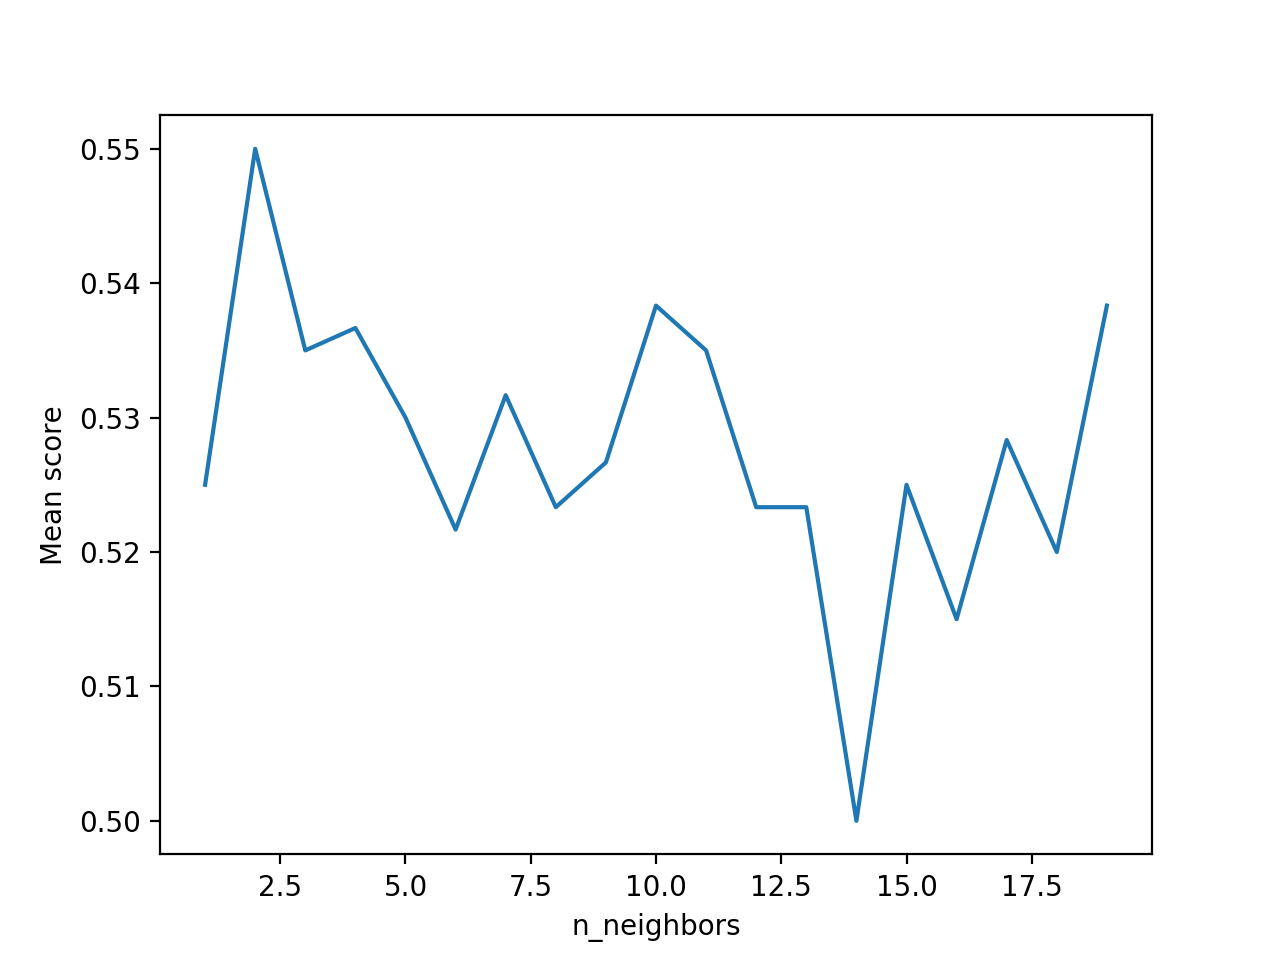
\includegraphics[width=5 in]{KNeighborsClassifier.png}
		\centering
		\caption{KNeighborsClassifier Tuning }
		\label{KN_t}
    		\end{figure}
		
\begin{figure}[!]
    		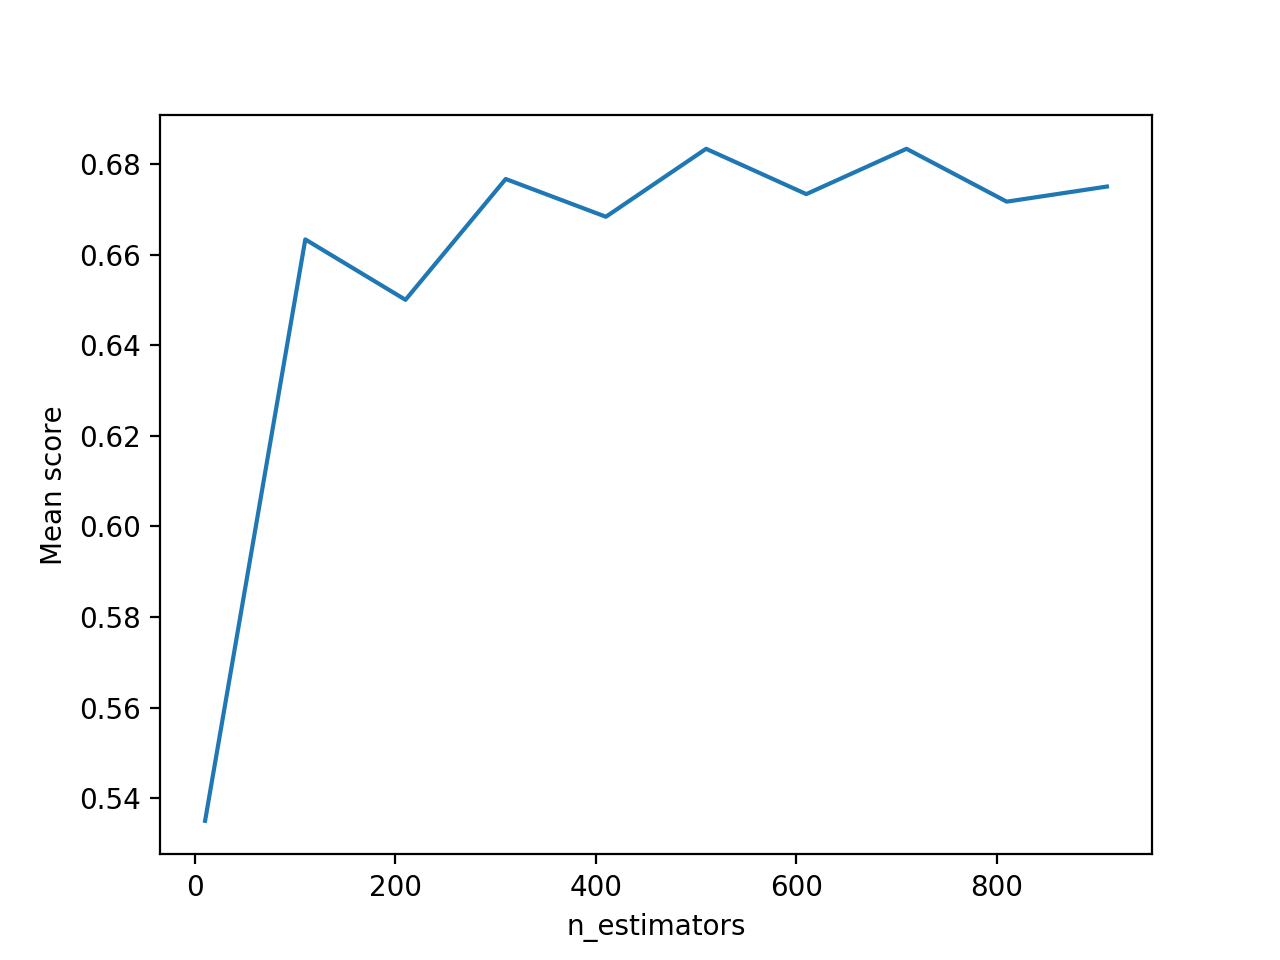
\includegraphics[width=5 in]{RandomForestClassifier.png}
		\centering
		\caption{RandomForestClassifier Tuning }
		\label{forest_t}
    		\end{figure}

\begin{figure}[!]
    		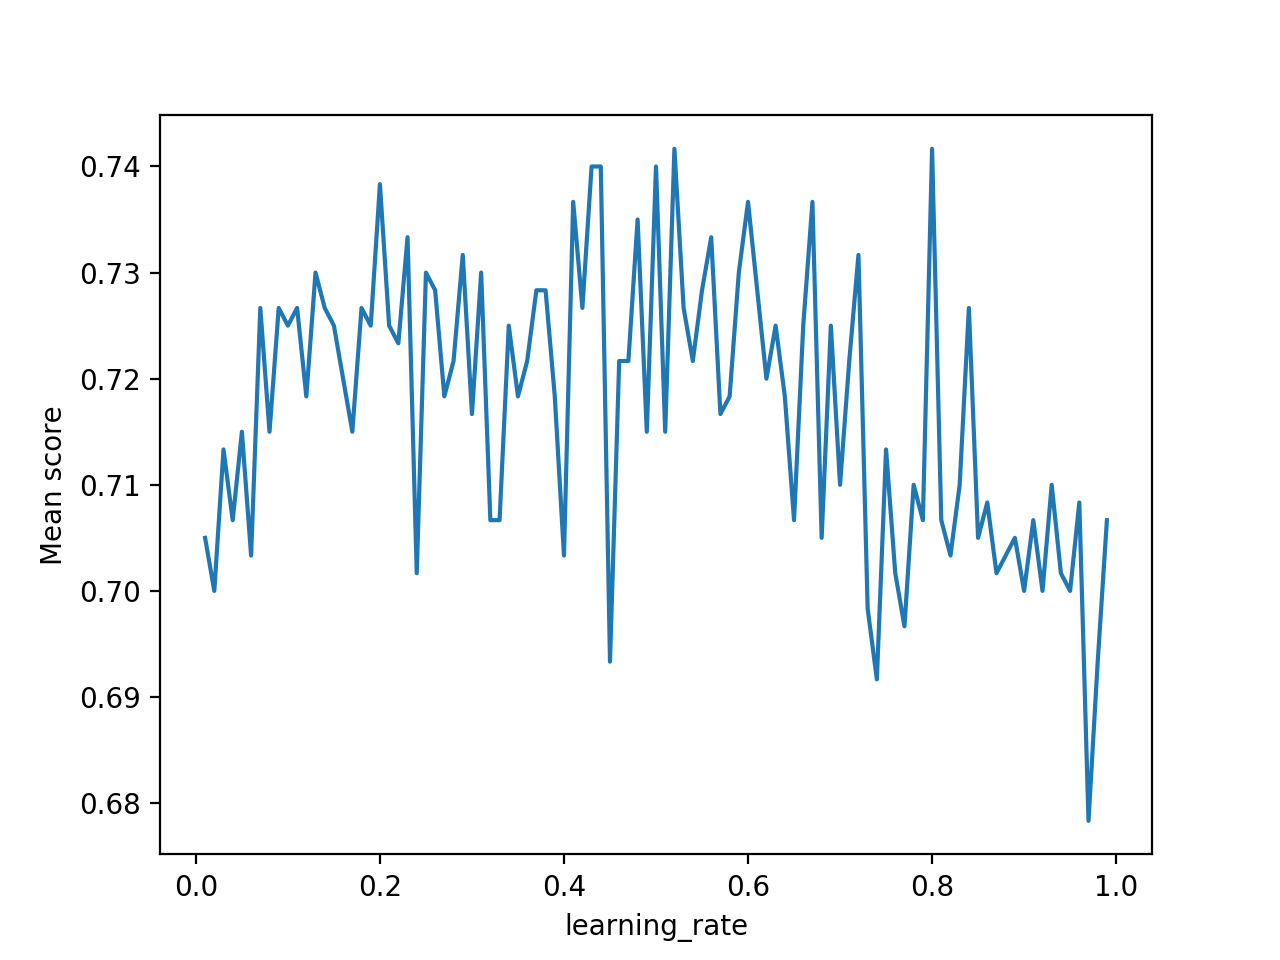
\includegraphics[width=5 in]{GradientBoostingClassifier.png}
		\centering
		\caption{GradientBoostingClassifier Tuning }
		\label{boost_t}
    		\end{figure}


\newpage
\section*{Supplementary File 2}	
This part includes all codes.

\textbf{Python Codes of Final Project:}
\lstinputlisting[language=Python]{Proj4.py}	


\renewcommand\refname{Reference}
\bibliographystyle{unsrt}
\bibliography{/Users/ccai28/Desktop/CS/ML/Project4/ref}









\end{document}
